\section{Experiments}


We evaluate OPD and OPSD on reasoning, system-prompt internalization, and alignment, covering both failure and success regimes.

\subsection{Math Reasoning}



\paragraph{OPSD.}

We train Qwen3-1.7B on OpenThoughts using stopgrad Top20 reverse KL (Equation \ref{eq:topksgKL}), with the step-0 checkpoint as the PI-conditioned teacher. We keep English problems with verifiable boxed answers. As shown in Figure~\ref{fig:2opsdfails}, neither answer-only nor full-response PI makes stable improvements on Math500, AIME24, or AIME25. Full-response PI performs worse than answer-only
PI, suggesting that richer PI can increase mismatch rather than improve
supervision. We further test whether this failure is due to a weak
PI-conditioned teacher by training a Qwen3-1.7B teacher with GRPO under
full-response PI (purple line in Figure~\ref{fig:2opsdfails}). This RL-trained teacher performs even worse, indicating that
PI alone does not make math OPSD effective.





\paragraph{OPD.}We use a Qwen3-1.7B student and a Qwen3-8B teacher, both with thinking mode disabled, trained on OpenThoughts with an unnormalized Top20 reverse-KL objective (Figure~\ref{fig:3opdcollapse}). OPD initially improves but later collapses. Around step 700, rollout length and revision tokens such as ``wait'' and ``maybe'' increase sharply; by step 1000, the model degenerates into repetitive ``maybe'' outputs and accuracy on Math500, AIME24, and AIME25 drops nearly to zero. Token statistics show a corresponding abrupt rise in repetition and a collapse of teacher-student
overlap.


\begin{figure}[t]
    \centering
    \begin{subfigure}[t]{0.32\textwidth}
        \centering
        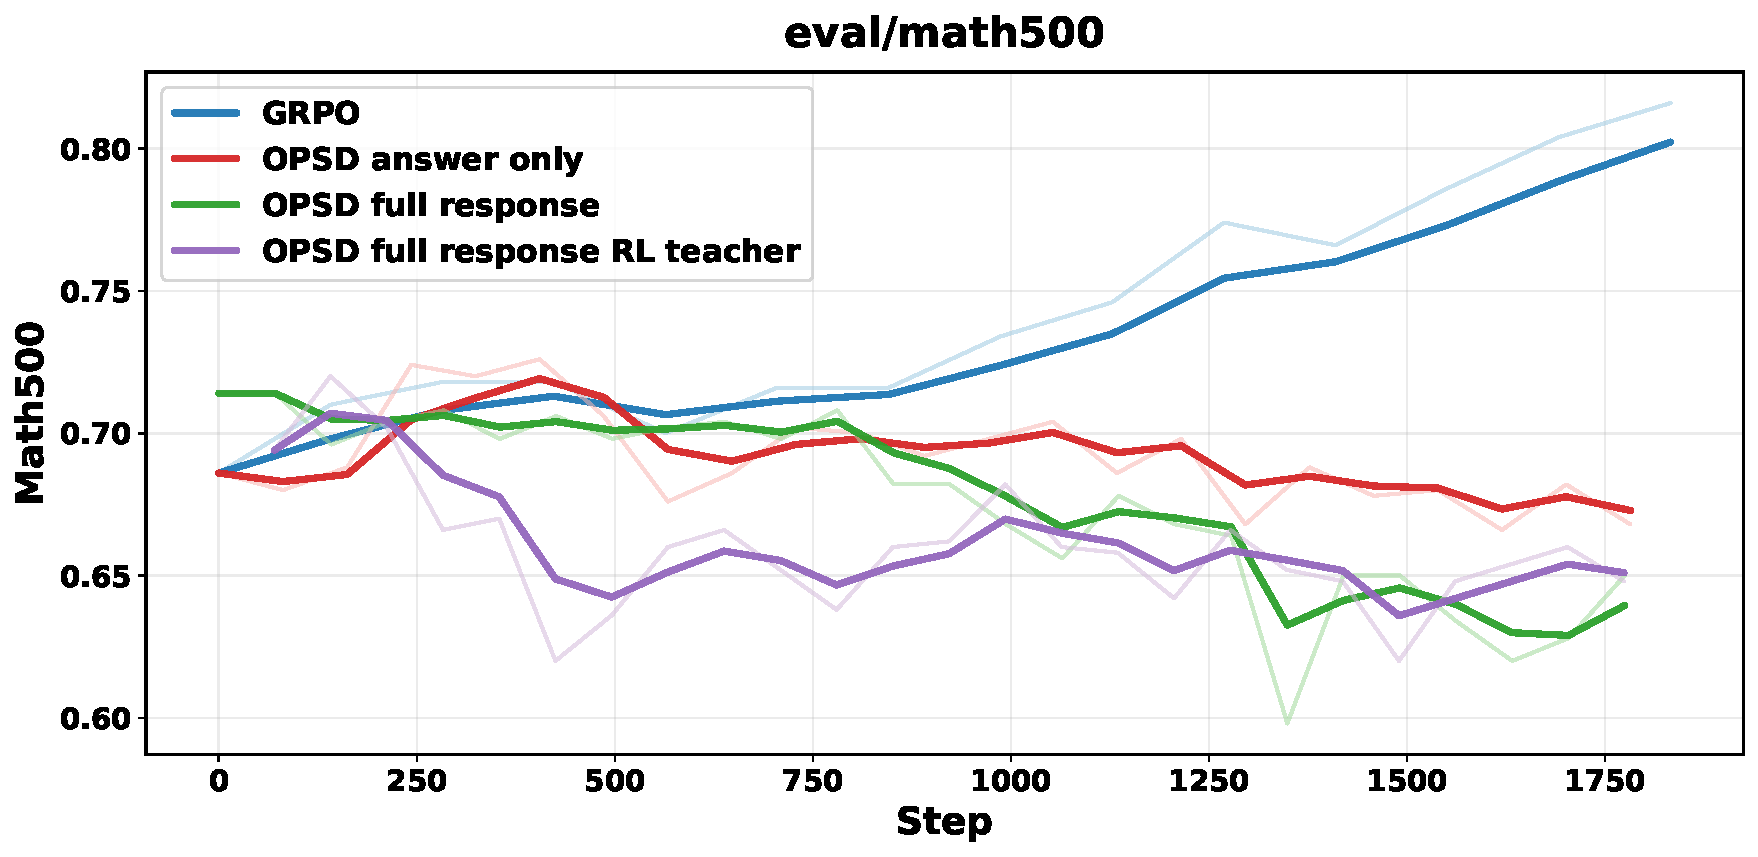
\includegraphics[width=\textwidth]{figures/top20_eval_math500_1.pdf}
        \label{fig:first}
    \end{subfigure}
    % \hfill
    \begin{subfigure}[t]{0.33\textwidth}
        \centering
        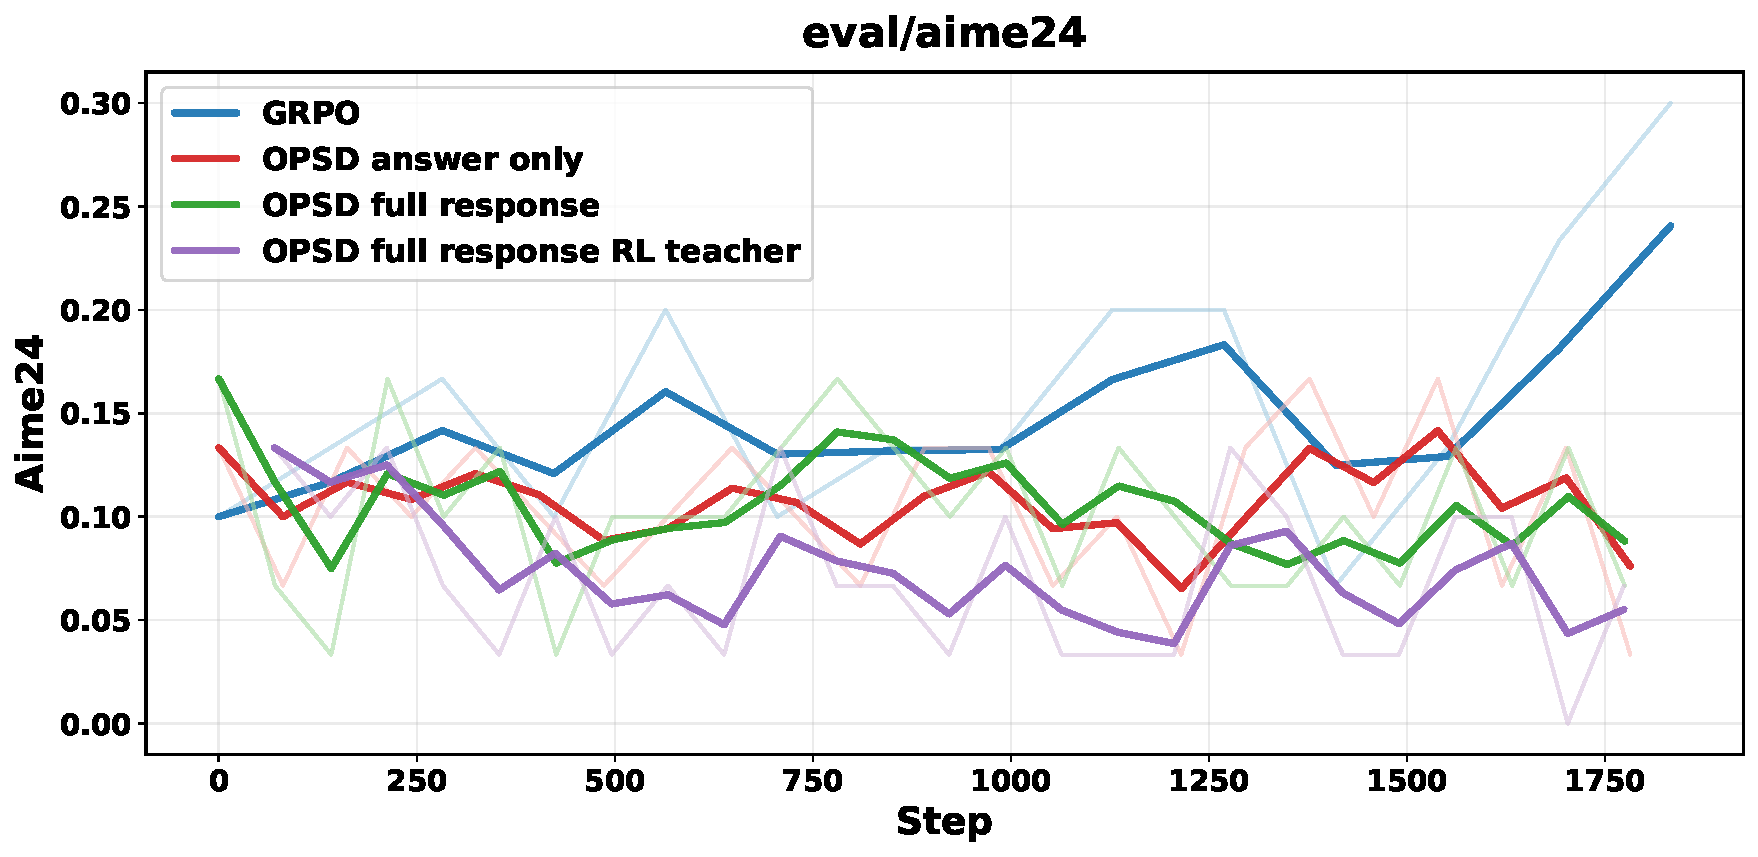
\includegraphics[width=\textwidth]{figures/top20_eval_aime24.pdf}
        \label{fig:second}
    \end{subfigure}
    \begin{subfigure}[t]{0.33\textwidth}
        \centering
        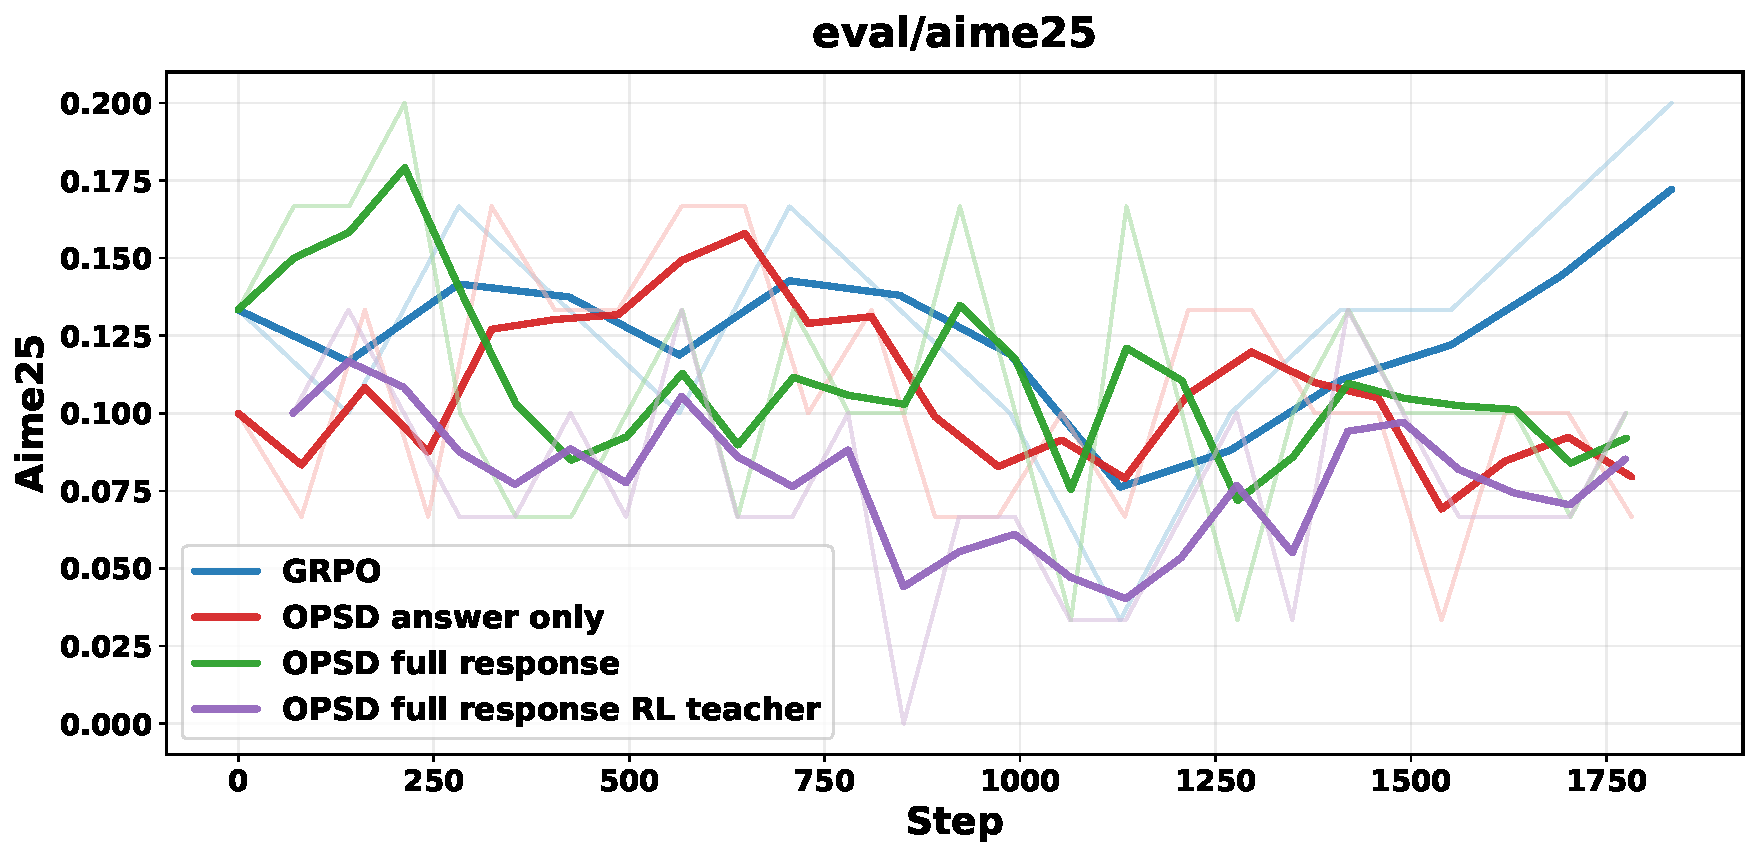
\includegraphics[width=\textwidth]{figures/top20_eval_aime25.pdf}
        \label{fig:second}
    \end{subfigure}
    % \begin{subfigure}[t]{0.24\textwidth}
    %     \centering
    %     \includegraphics[width=\textwidth]{figures/top20_response_lengths_1.pdf}
    %     \label{fig:second}
    % \end{subfigure}
    \vspace{-3mm}
    \caption{Qwen3-1.7B, trained on OpenThoughts. OPSD fails to improve student.}
    \label{fig:2opsdfails}
\end{figure}


\begin{figure}[t]
    \centering
    \begin{subfigure}[t]{0.3\textwidth}
        \centering
        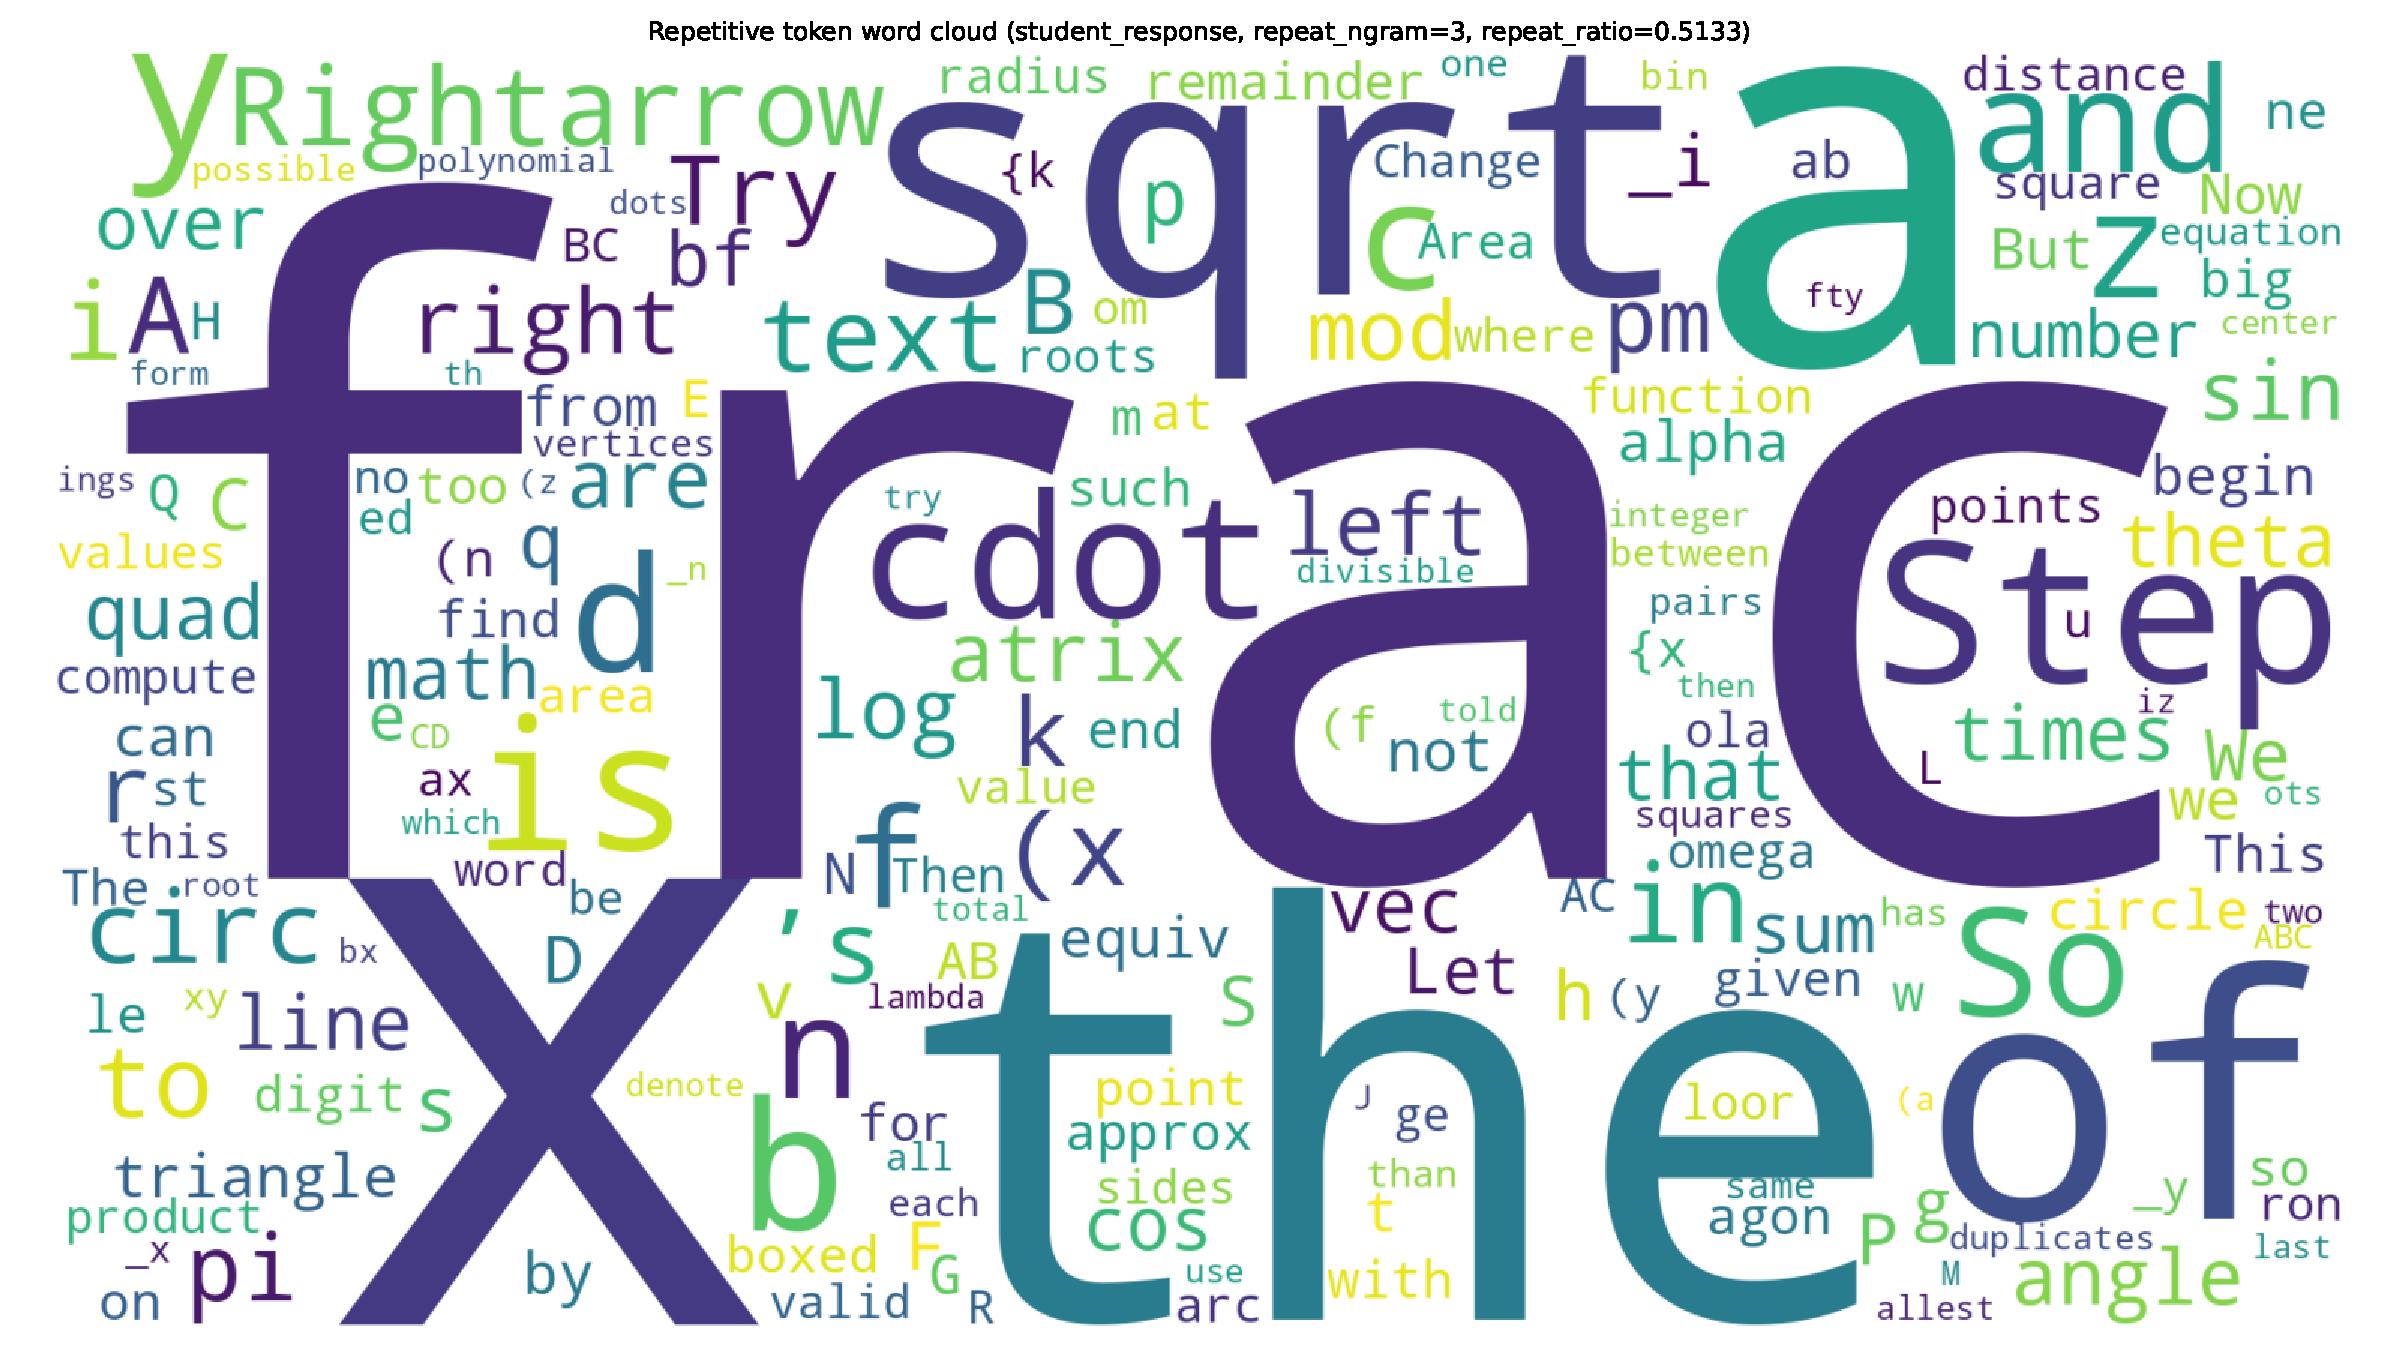
\includegraphics[width=\textwidth]{figures/eval_0_student_response_repeat_ngram3_wordcloud.pdf}
        \caption{step0}
        \label{fig:step0}
    \end{subfigure}
    \hfill
    \begin{subfigure}[t]{0.3\textwidth}
        \centering
        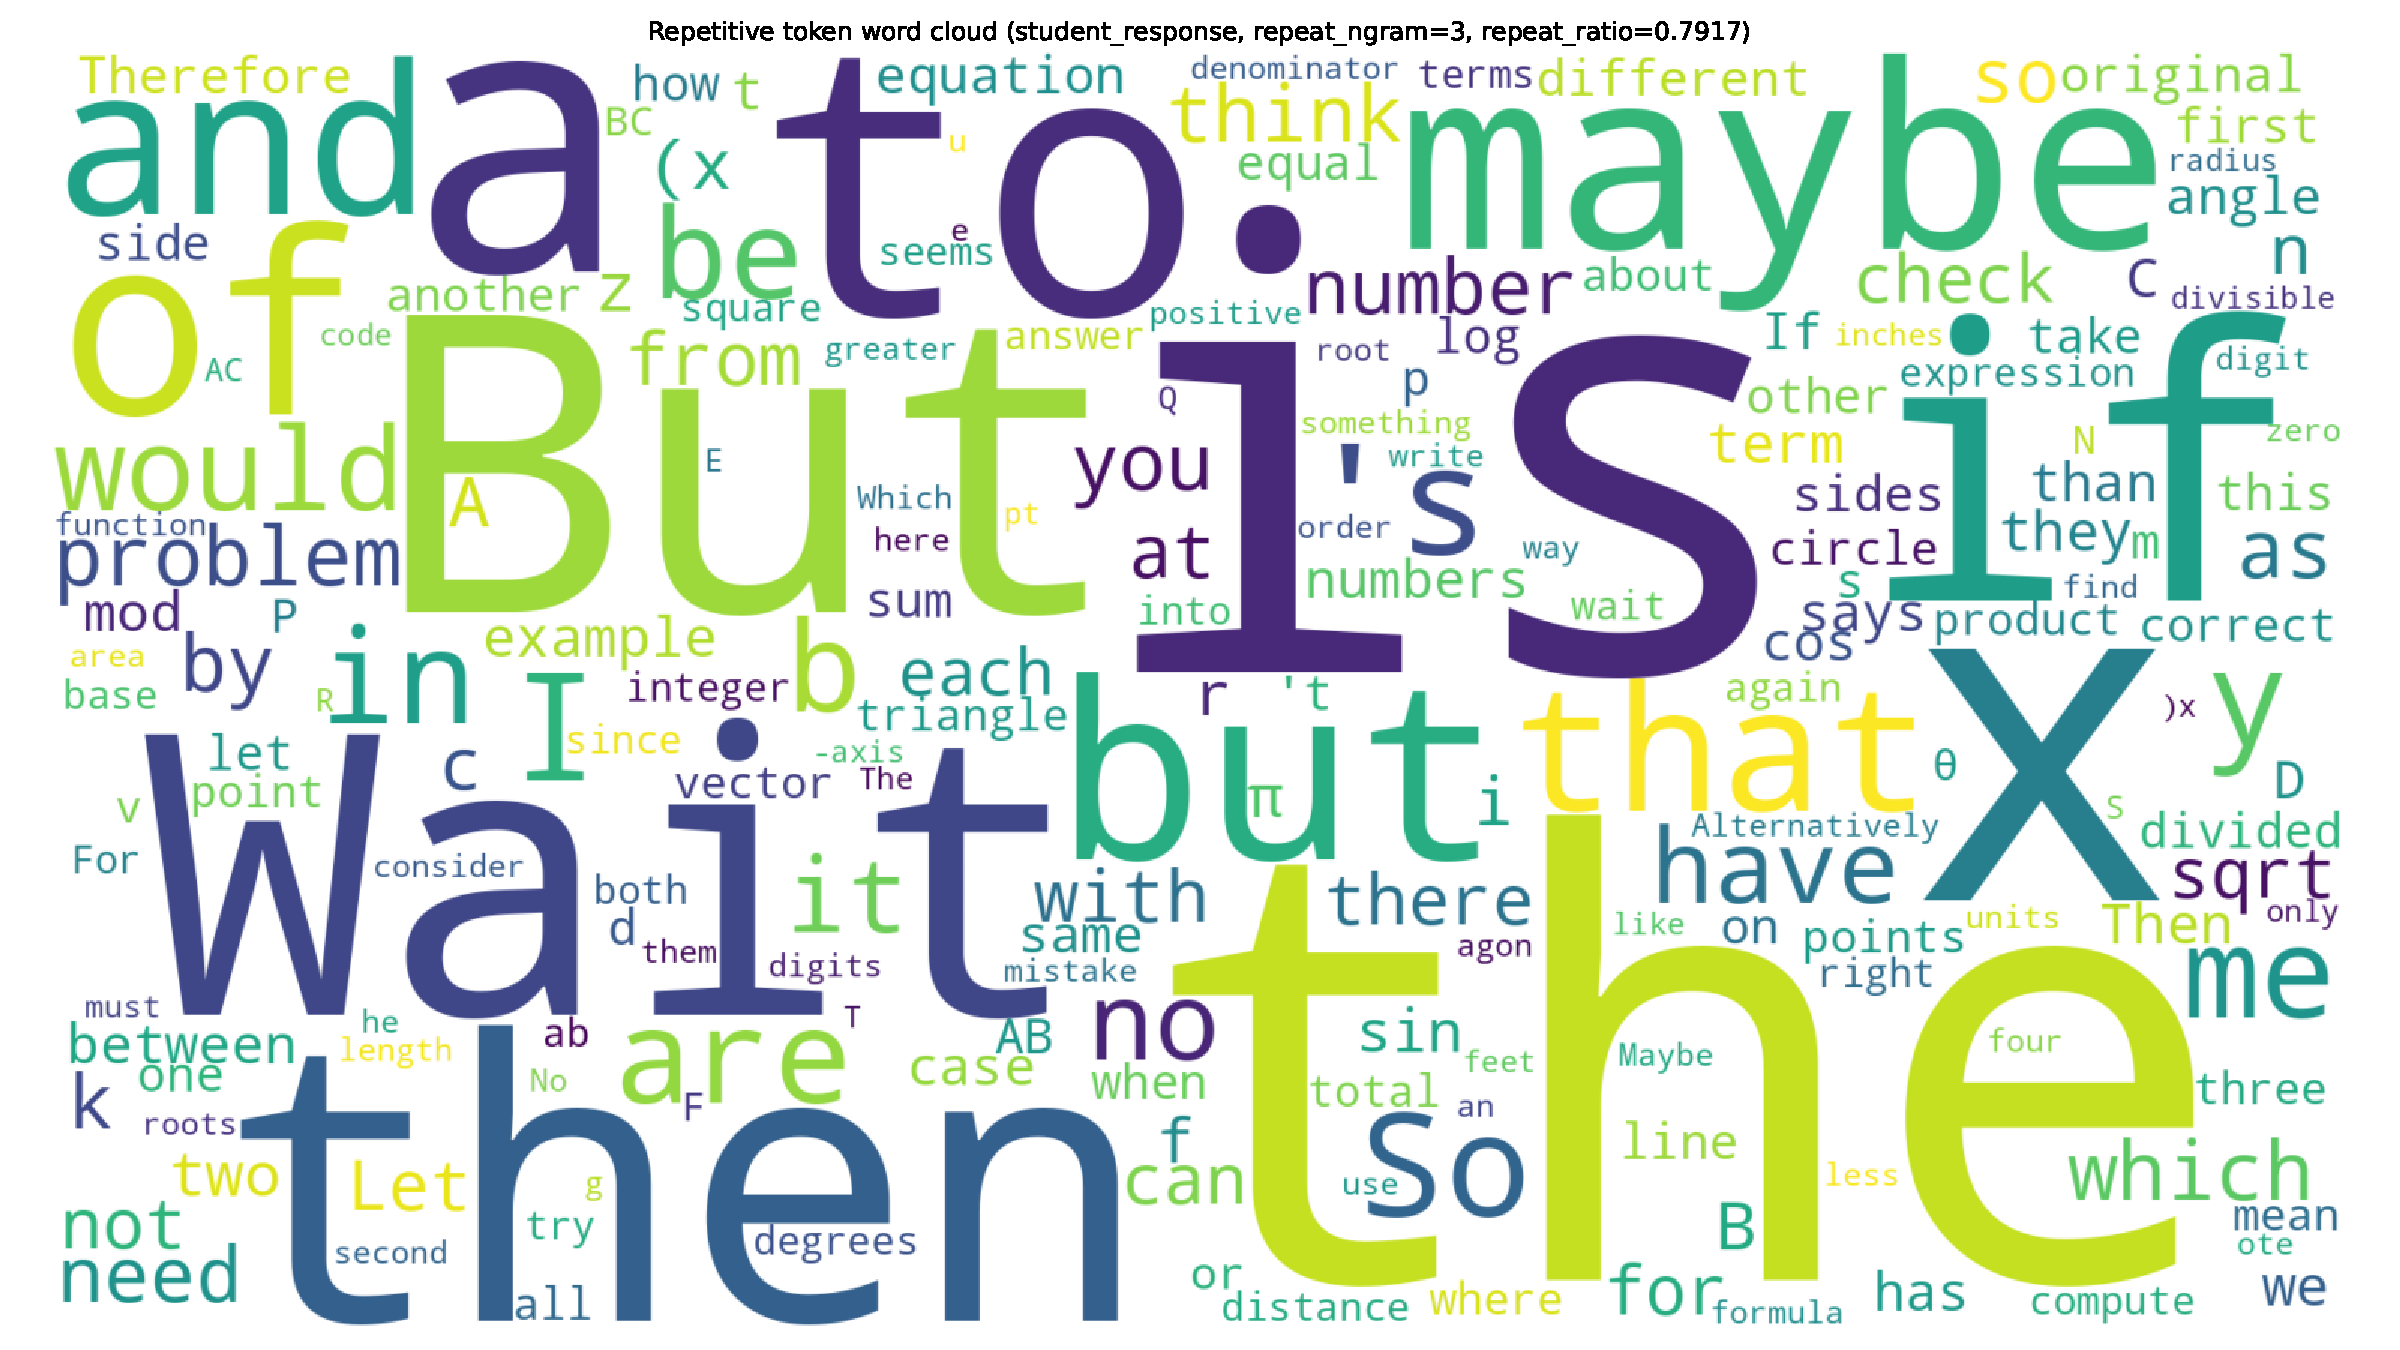
\includegraphics[width=\textwidth]{figures/eval_119_student_response_repeat_ngram3_wordcloud.pdf}
        \caption{step700}
        \label{fig:step700}
    \end{subfigure}
    \hfill
    \begin{subfigure}[t]{0.3\textwidth}
        \centering
        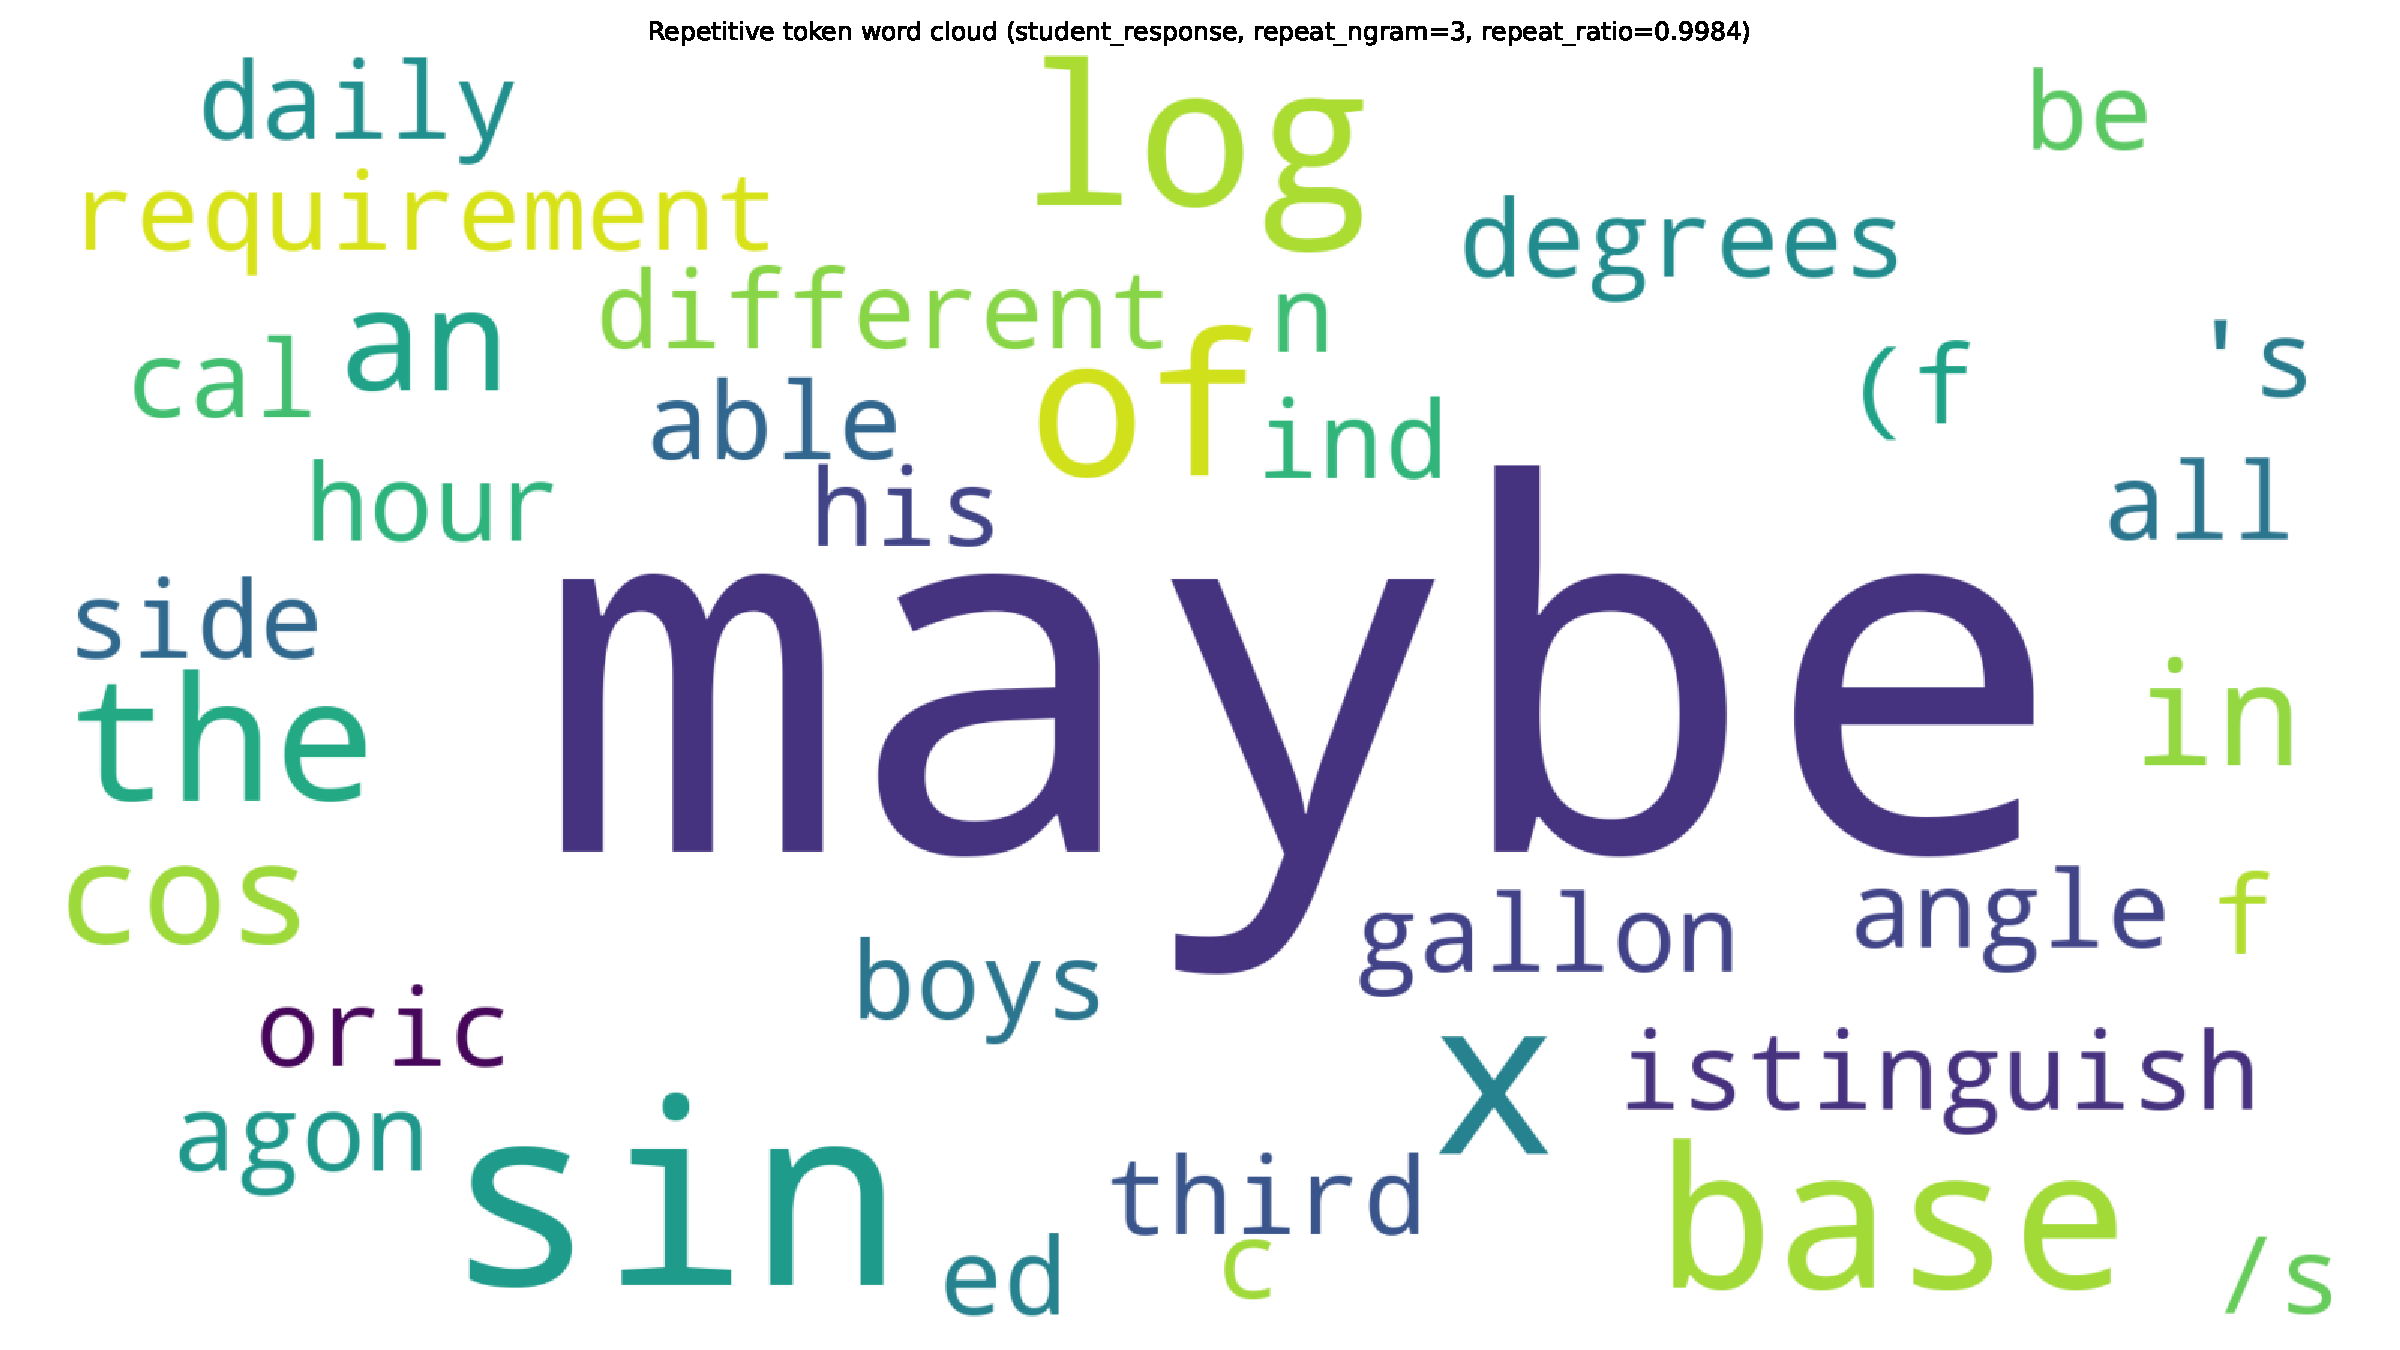
\includegraphics[width=\textwidth]{figures/eval_149_student_response_repeat_ngram3_wordcloud.pdf}
        \caption{step1000}
        \label{fig:step1000}
    \end{subfigure}

    \centering
    \begin{subfigure}[t]{0.3\textwidth}
        \centering
        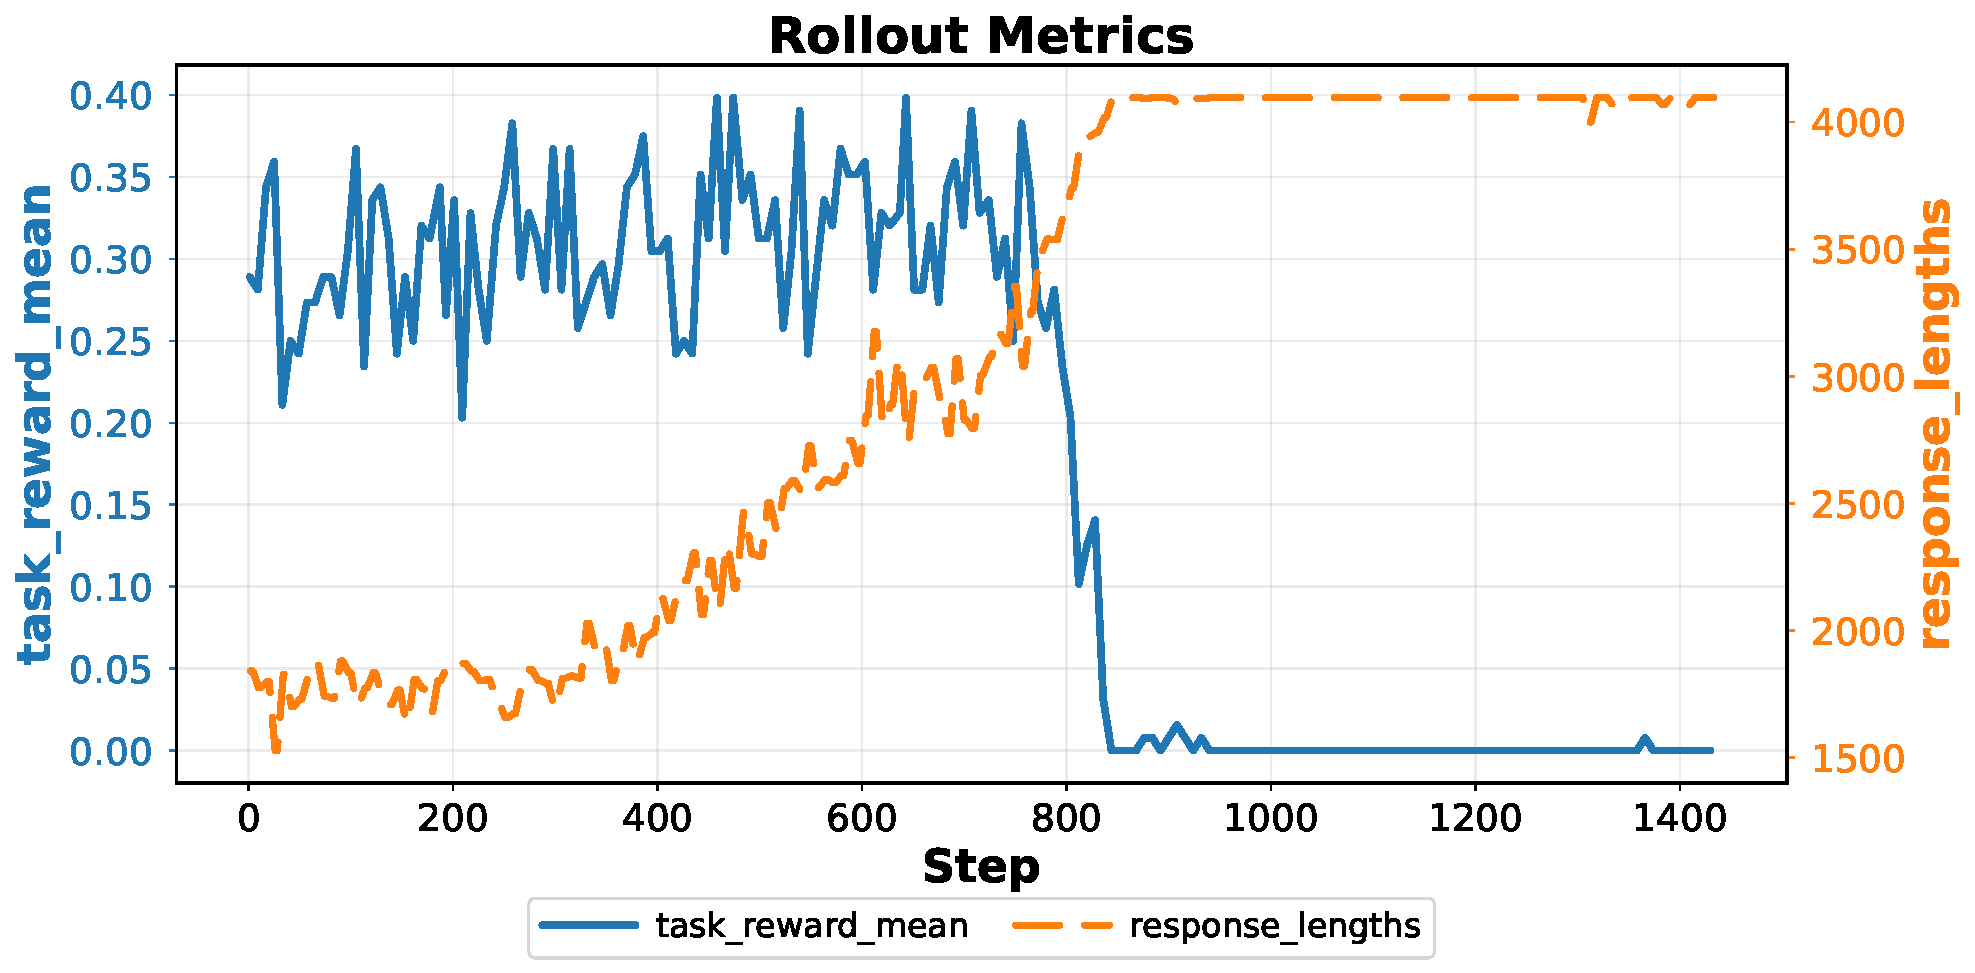
\includegraphics[width=\textwidth]{figures/rollout_metrics_dual_axis.pdf}
        \caption{rollout metrics}
        \label{fig:rollout_metrics}
    \end{subfigure}
    \hfill
    \begin{subfigure}[t]{0.35\textwidth}
        \centering
        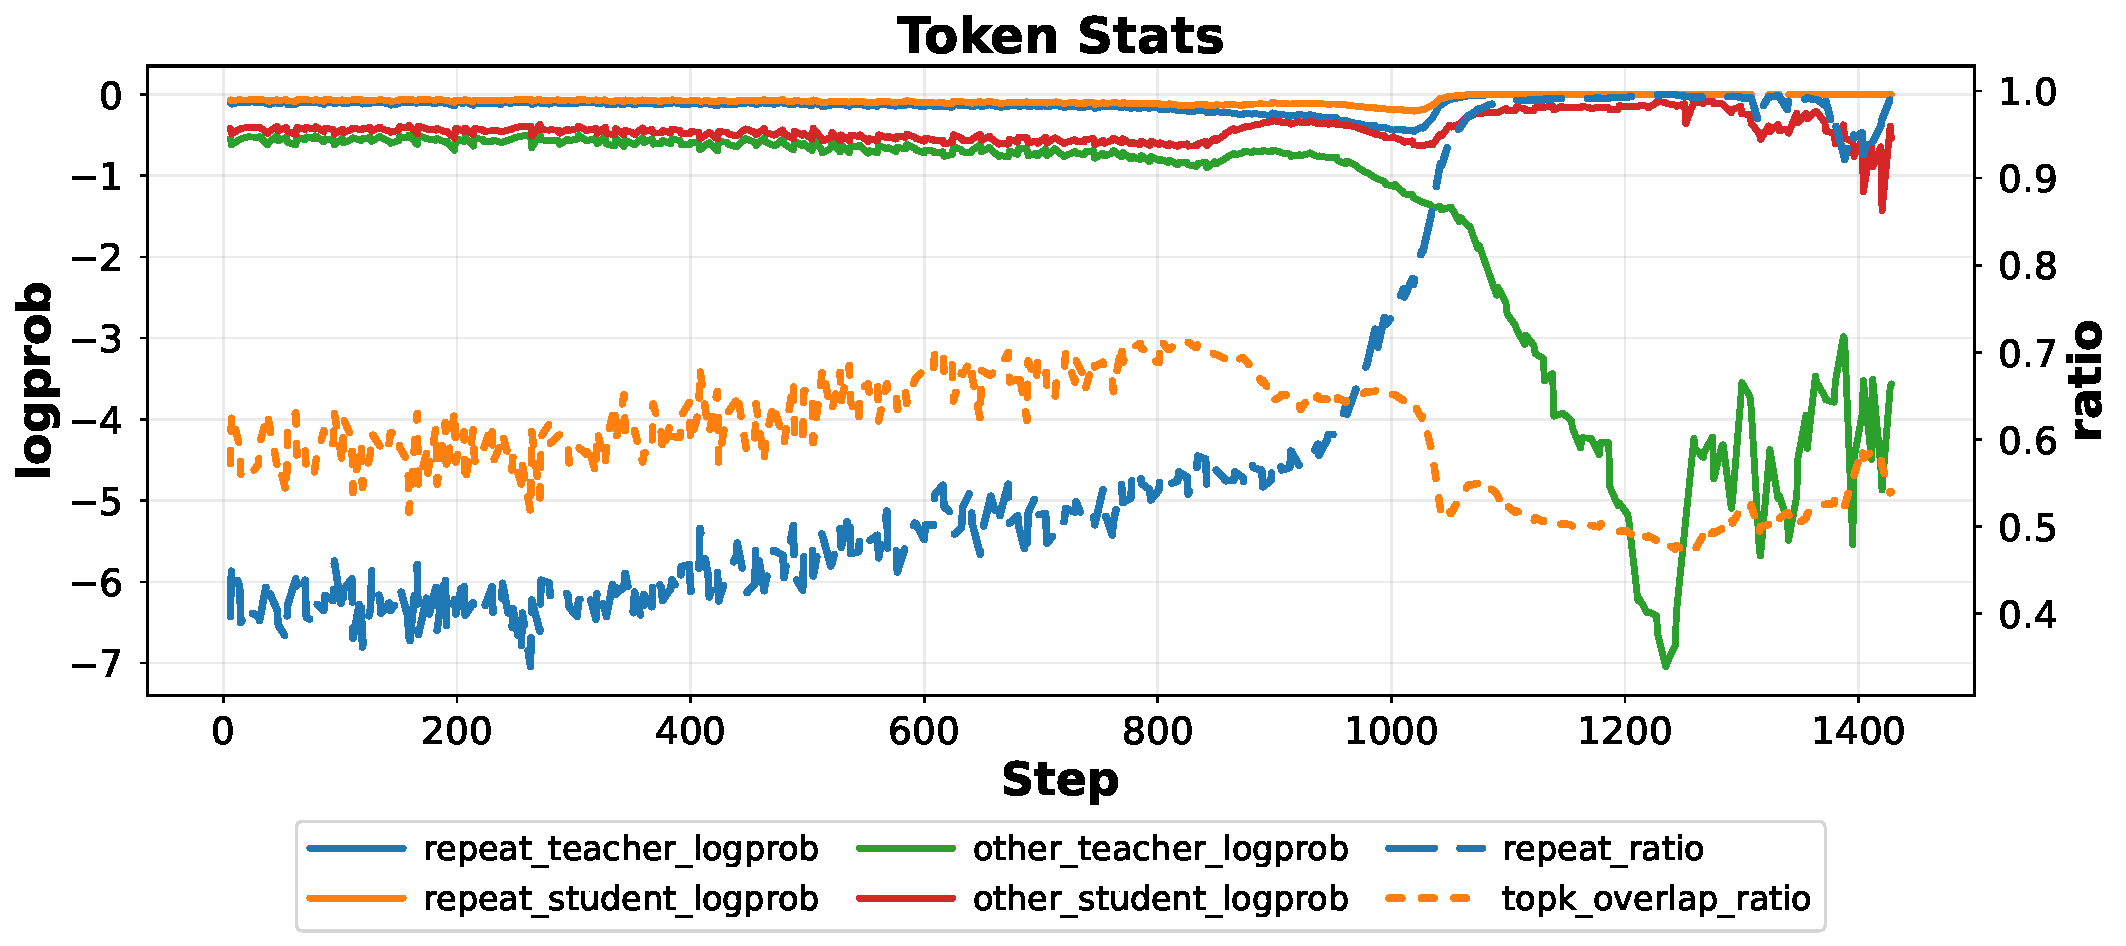
\includegraphics[width=\textwidth]{figures/opd_token_stats_dual_axis.pdf}
        \caption{token stats}
        \label{fig:token_stats}
    \end{subfigure}
    \hfill
    \begin{subfigure}[t]{0.3\textwidth}
        \centering
        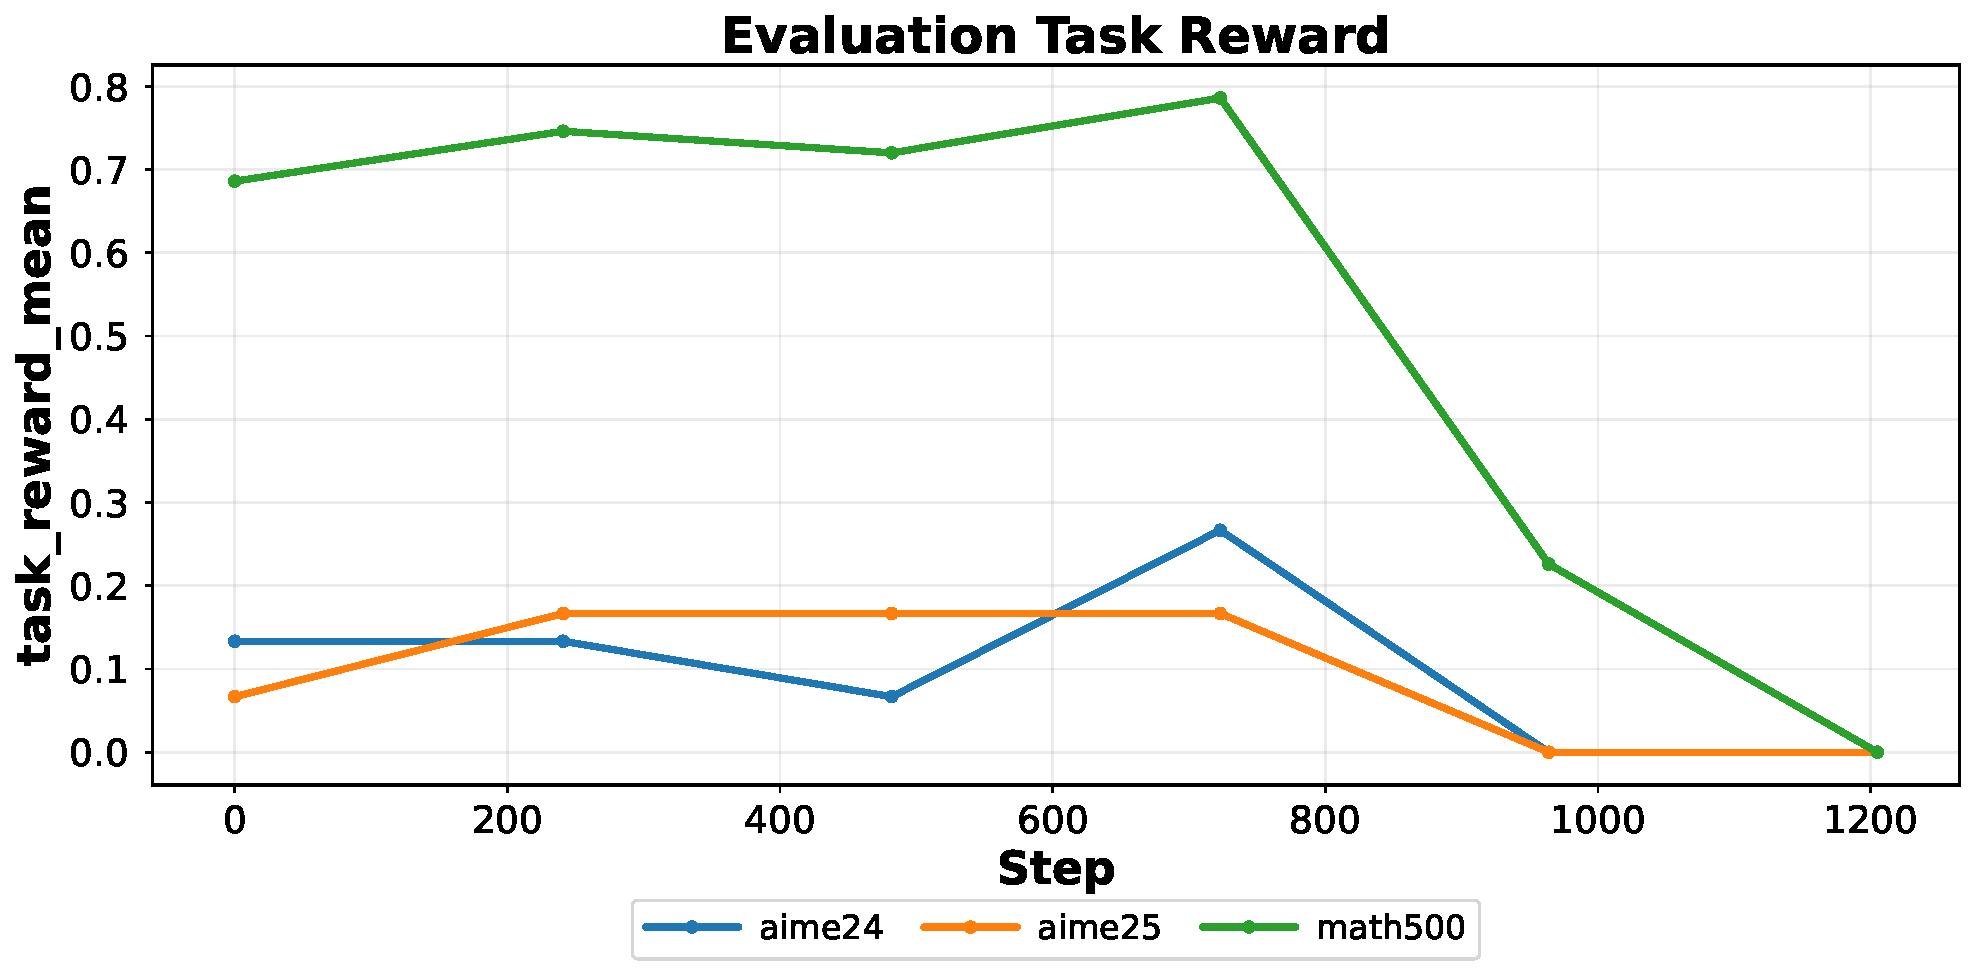
\includegraphics[width=\textwidth]{figures/eval_task_reward_metrics.pdf}
        \caption{eval acc}
        \label{fig:eval_acc}
    \end{subfigure}
    
    \caption{
    % (\textbf{a-c}) Word clouds of response patterns: At step 700, the student shows increased verbosity, with filler words such as “wait”, “but”, and “maybe”. By step 1000, the model collapses into severe repetition, producing “maybe” excessively. (\textbf{d}) shows a sharp decline in reward as response lengths hit the ceiling. (\textbf{e}) The log-probabilities of repetitive tokens (repeat\_*\_logprob) remain significantly higher than non-repetitive ones (other\_*\_logprob), while the repeat ratio reaches to nearly 1.0. (\textbf{f}) evaluation accuracy decreases because of length explosion.
    Collapse under unnormalized Top-$20$ reverse KL. The model first
    becomes verbose, then degenerates into repetitive ``maybe'' outputs as response
    length reaches the limit and evaluation accuracy drops. Token statistics show that repetitive tokens dominate as the repeat ratio approaches one.
    }
    \label{fig:3opdcollapse}
\end{figure}



\subsection{Alignment \& System Prompt Internalization.}

\paragraph{Alignment.}We evaluate OPSD on two style-alignment benchmarks: CharacterBench~\cite{zhou2024characterbenchbenchmarkingcharactercustomization} and EmotionBench~\cite{huang2024emotionallynumbempatheticevaluating}.
For both tasks, we provide the teacher with a question-specific alignment prompt as privileged information; details are provided in Appendix~\ref{app:style_pi}.
We compare OPSD with GRPO and PPO using Qwen3-4B-Instruct and Qwen3-8B students.
As shown in Figure~\ref{fig:style_alignment}, under the same sampling budget, OPSD improves and converges faster than both RL baselines.


\begin{figure}[t]
    \centering
    \begin{subfigure}[t]{0.48\textwidth}
        \centering
        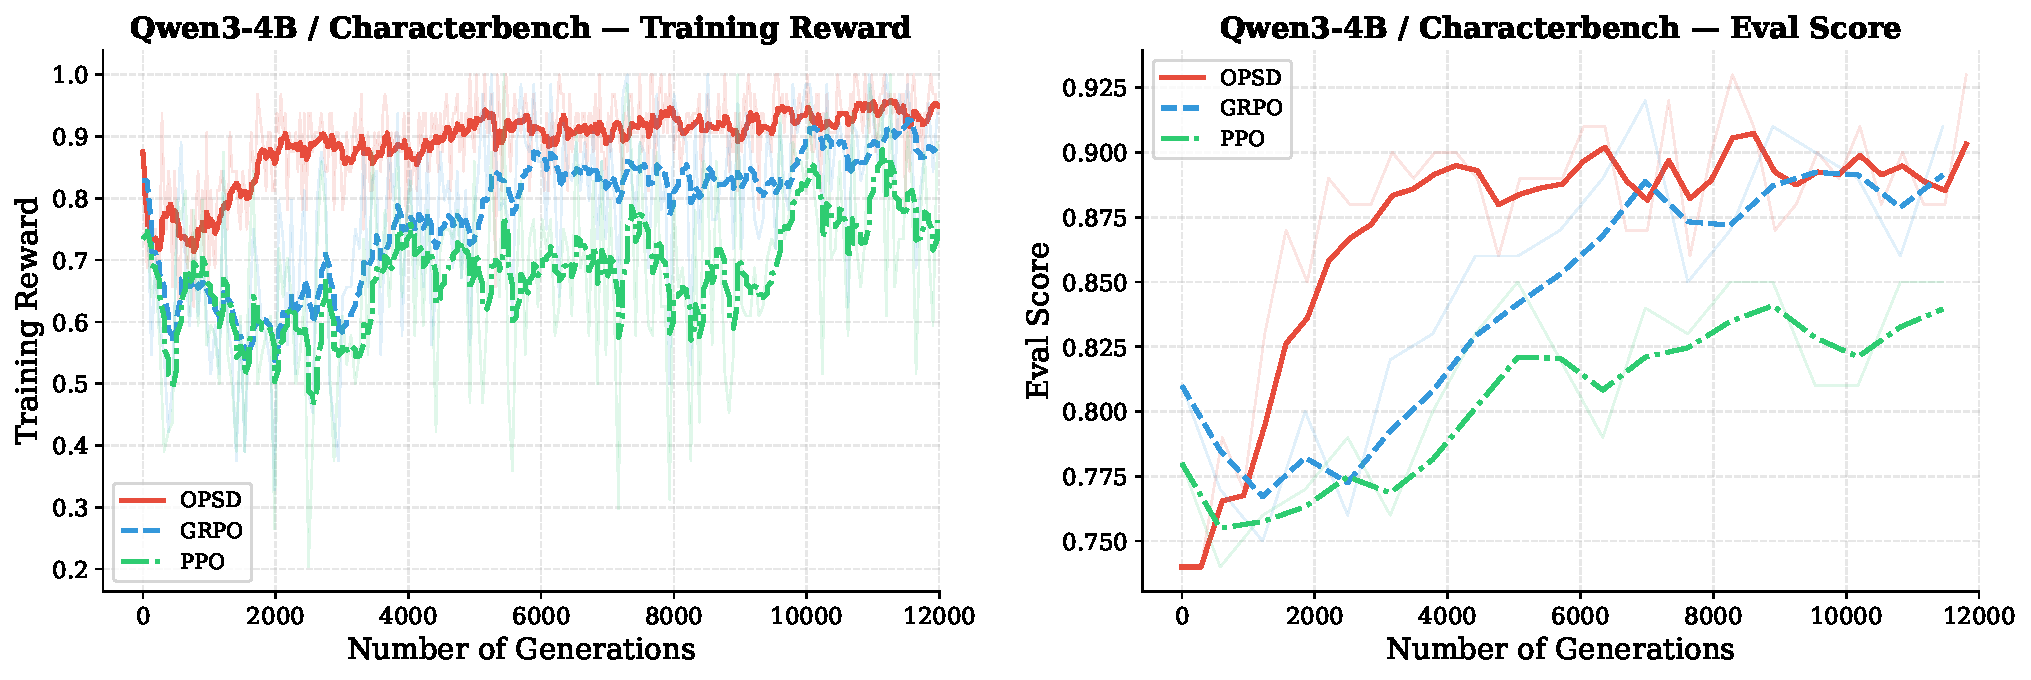
\includegraphics[width=\textwidth]{figures/qwen3-4B_characterbench.pdf}
        % \caption{Qwen3-4B on CharacterBench}
        \label{fig:4b_char}
    \end{subfigure}
    \hfill
    \begin{subfigure}[t]{0.48\textwidth}
        \centering
        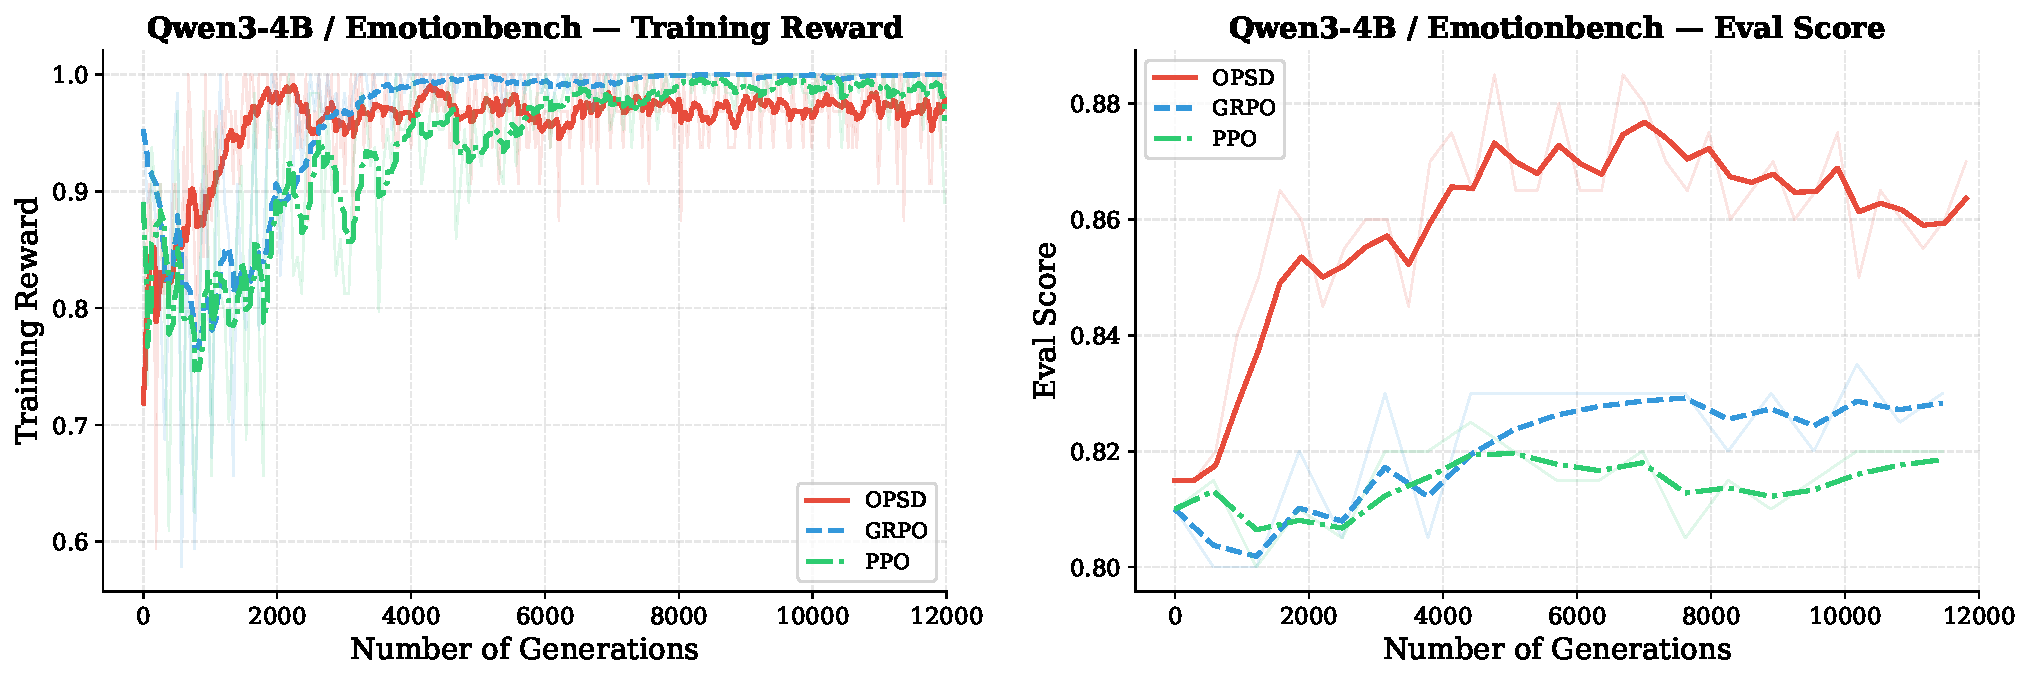
\includegraphics[width=\textwidth]{figures/qwen3-4B_emotionbench.pdf}
        % \caption{Qwen3-4B on EmotionBench}
        \label{fig:4b_emo}
    \end{subfigure}
    % \vspace{0.5em}
    % \begin{subfigure}[t]{0.48\textwidth}
    %     \centering
    %     \includegraphics[width=\textwidth]{figures/qwen3-8B_characterbench.pdf}
    %     \caption{Qwen3-8B on CharacterBench}
    %     \label{fig:8b_char}
    % \end{subfigure}
    % \hfill
    % \begin{subfigure}[t]{0.48\textwidth}
    %     \centering
    %     \includegraphics[width=\textwidth]{figures/qwen3-8B_emotionbench.pdf}
    %     \caption{Qwen3-8B on EmotionBench}
    %     \label{fig:8b_emo}
    % \end{subfigure}
    \vspace{-3mm}
    \caption{Training reward (left) and evaluation score (right) curves for OPSD, GRPO, and PPO on CharacterBench and EmotionBench, using Qwen3-4B-Instruct as student models.
    % Training reward (left) and evaluation score (right) curves for OPSD, GRPO, and PPO on CharacterBench and EmotionBench, using Qwen3-4B-Instruct (top) and Qwen3-8B (bottom) as student models.
    }
    \label{fig:style_alignment}
\end{figure}



\paragraph{System Prompt Internalization.} We next study two applications of system prompt internalization: reasoning compression and safety alignment on adversarial questions. In contrast to the alignment tasks above, where the privileged information is question-specific, system prompt internalization uses a fixed system prompt as privileged information for all questions. For reasoning compression, shown in Figure~\ref{fig:opsdc_vs_grpo}, OPSD does not harm accuracy while substantially reducing response length. Compared with GRPO using a length penalty, OPSD is more sample efficient. It also offers a practical efficiency advantage: RL requires a large generation length to get a final answer, but OP(S)D can use shorter rollouts because the supervision is provided token-wise. However, we find that this application requires a sufficiently capable model, such as an 8B-scale model, to be effective. This finding is also consistent with \cite{sang2026crispcompressedreasoningiterative}. The second application is safety alignment. We conduct experiments with Qwen3-1.7B and Wildguardmix dataset \cite{han2024wildguardopenonestopmoderation} using the system prompt in Appendix~\ref{app:opsd_alignment_prompt}, with results shown in Figure~\ref{fig:OPDonwildguard}. OPSD improves rapidly in the early stage of training, but its final performance is constrained by the teacher. In contrast, GRPO improves more gradually but continues to make gains after OPSD saturates.


\begin{figure*}[t]
    \centering

    \begin{minipage}[t]{0.3\textwidth}
        \centering
        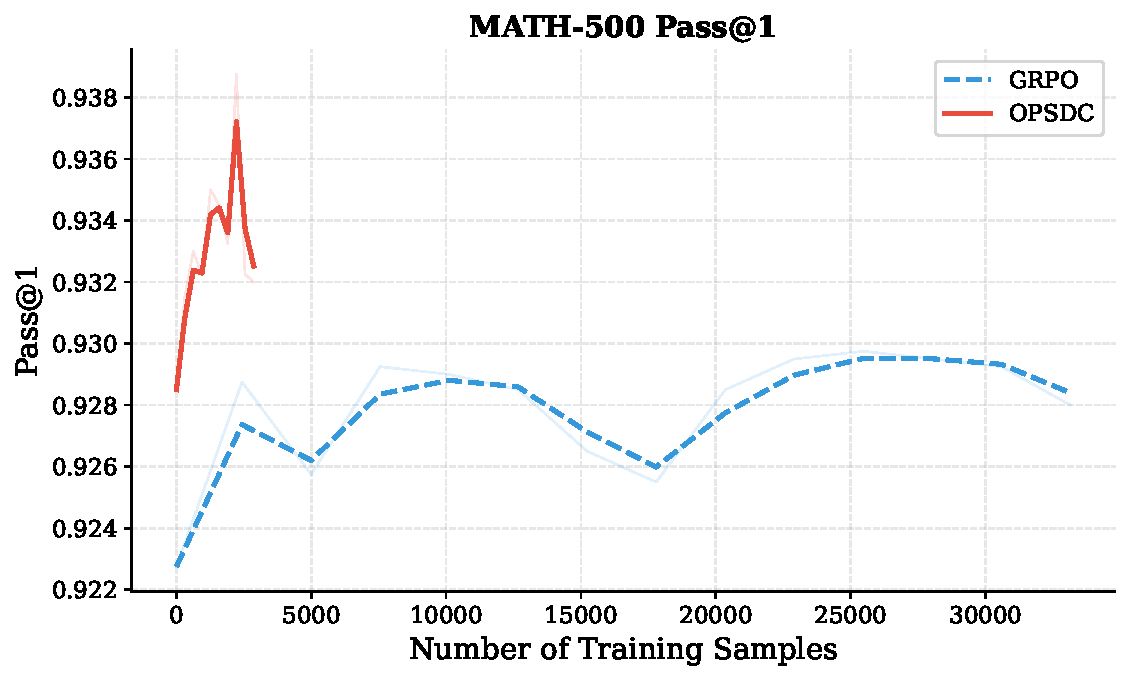
\includegraphics[width=\textwidth]{figures/opsdc_vs_grpo_pass1_eval.pdf}
        % \vspace{-0.5em}
        % \caption*{\small Eval Pass@1}
    \end{minipage}
    % \hfill
    % \begin{minipage}[t]{0.24\textwidth}
    %     \centering
    %     \includegraphics[width=\textwidth]{figures/opsdc_vs_grpo_pass1_train.pdf}
    %     \vspace{-0.5em}
    %     \caption*{\small Train reward}
    % \end{minipage}
    \hfill
    \begin{minipage}[t]{0.3\textwidth}
        \centering
        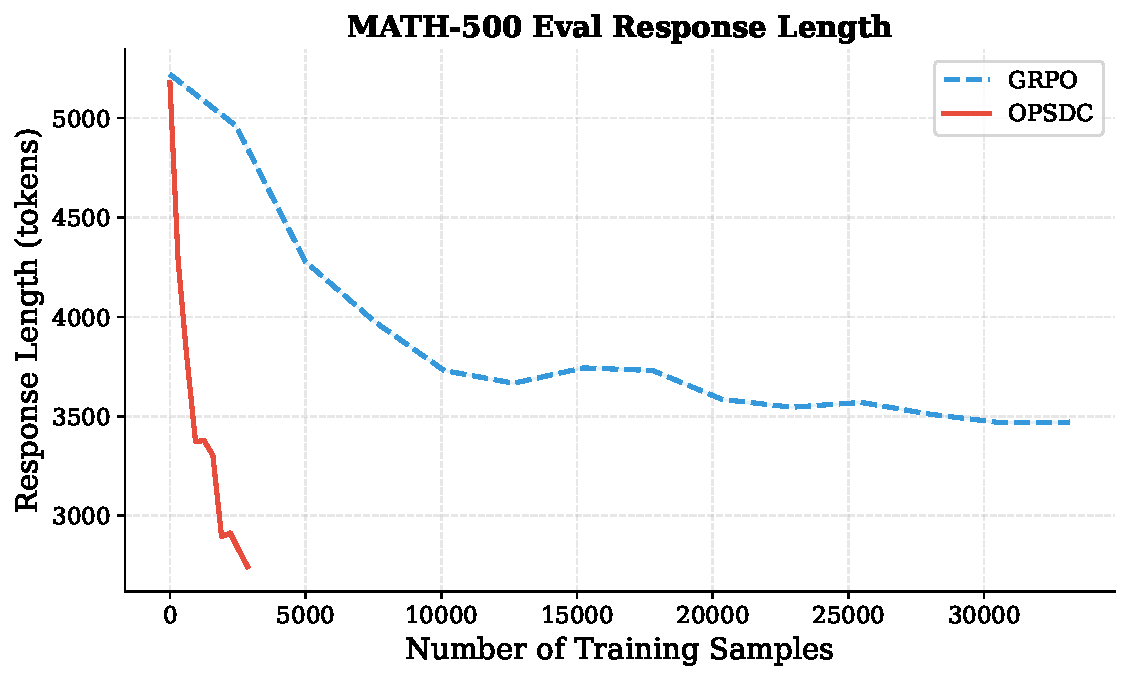
\includegraphics[width=\textwidth]{figures/opsdc_vs_grpo_resp_len_eval.pdf}
        % \vspace{-0.5em}
        % \caption*{\small Eval length}
    \end{minipage}
    \hfill
    \begin{minipage}[t]{0.3\textwidth}
        \centering
        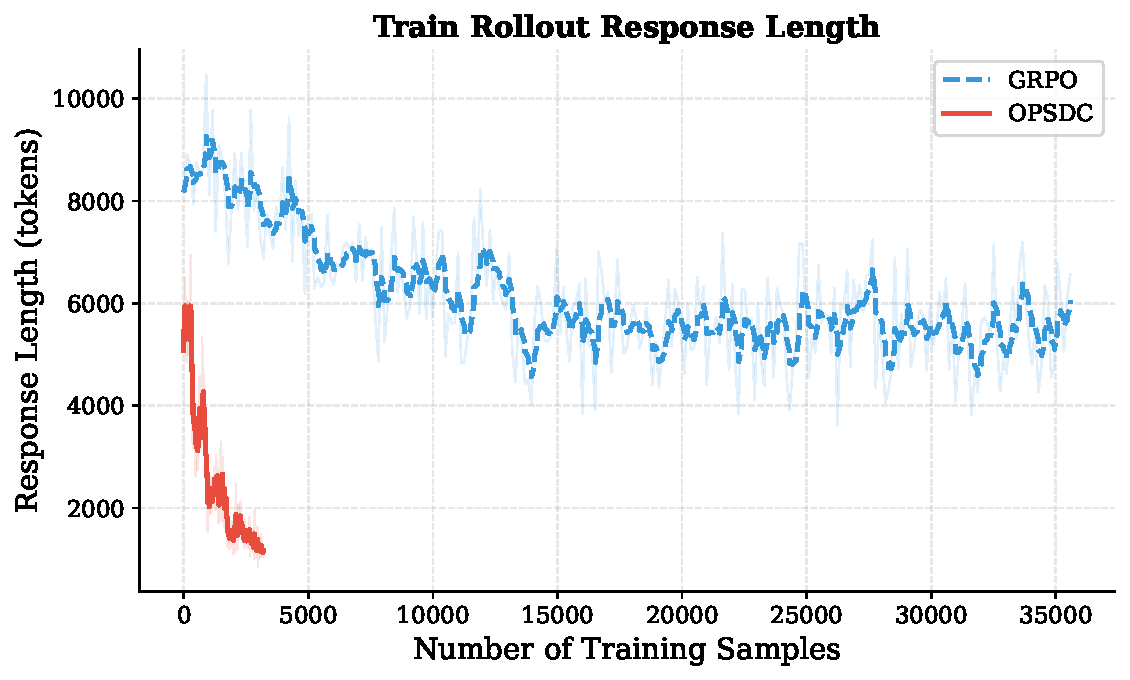
\includegraphics[width=\textwidth]{figures/opsdc_vs_grpo_resp_len_train.pdf}
        % \vspace{-0.5em}
        % \caption*{\small Train length}
    \end{minipage}
    % \vspace{-1mm}
    \caption{Comparison of GRPO and OPSD on Qwen3-8B (thinking mode) trained with DAPO-Math-17k~\cite{yu2025dapoopensourcellmreinforcement}.
    From left to right: MATH-500 Pass@1, evaluation response length, and training rollout response length.}
    \label{fig:opsdc_vs_grpo}
\end{figure*}


\begin{figure*}[t]
    \centering
    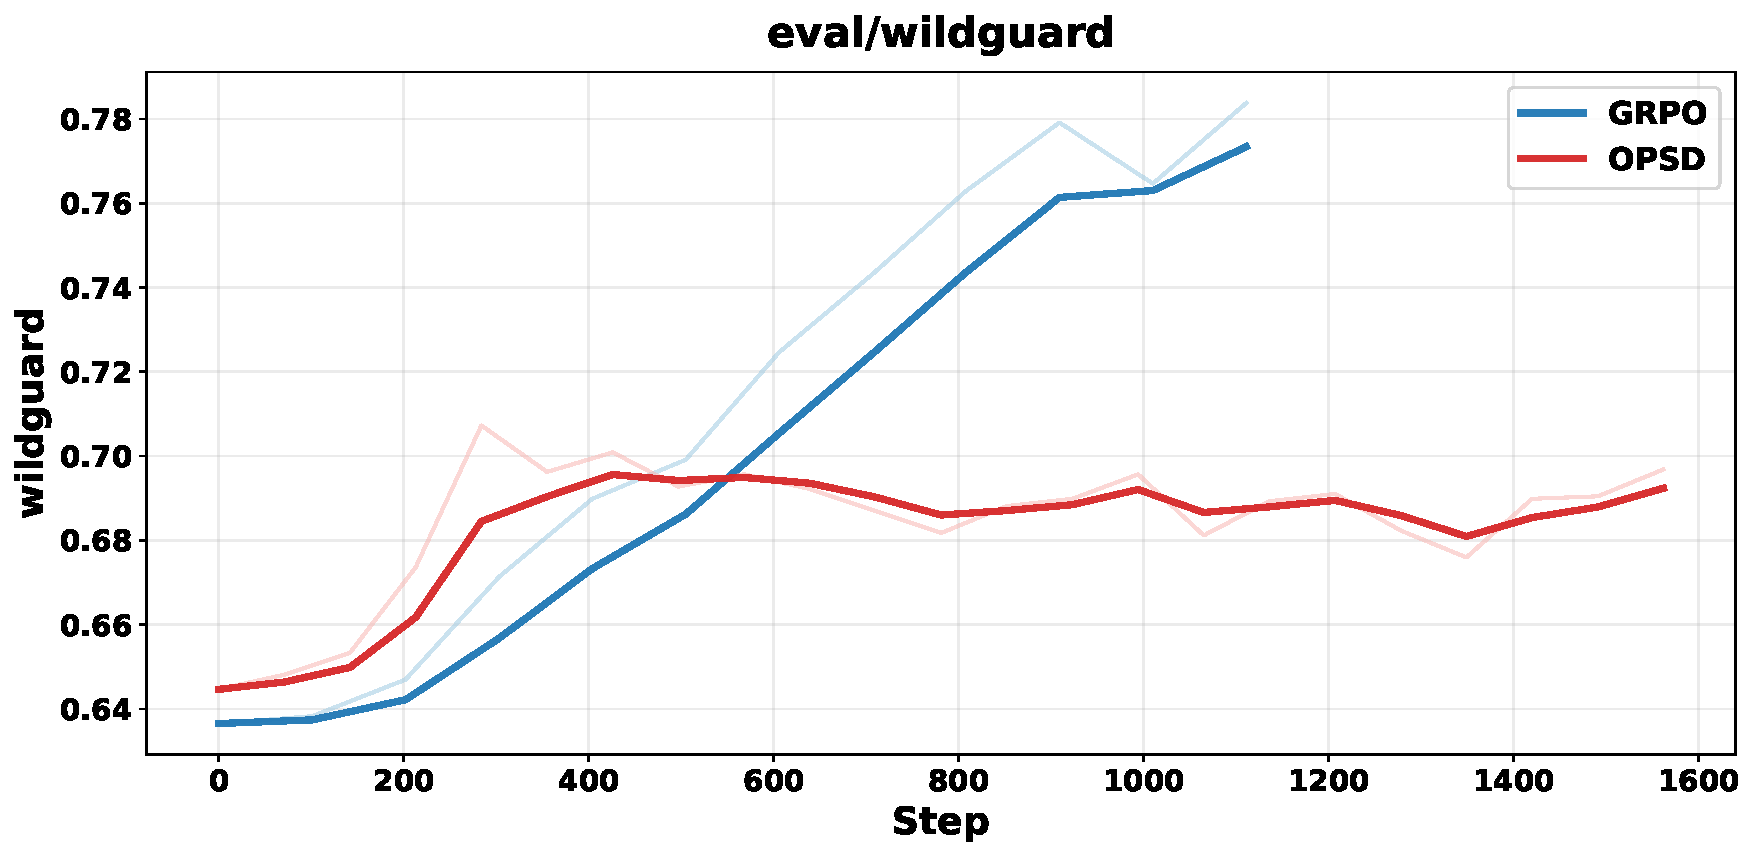
\includegraphics[width=0.3\textwidth]{figures/wildguard_eval.pdf}
    \hfill
    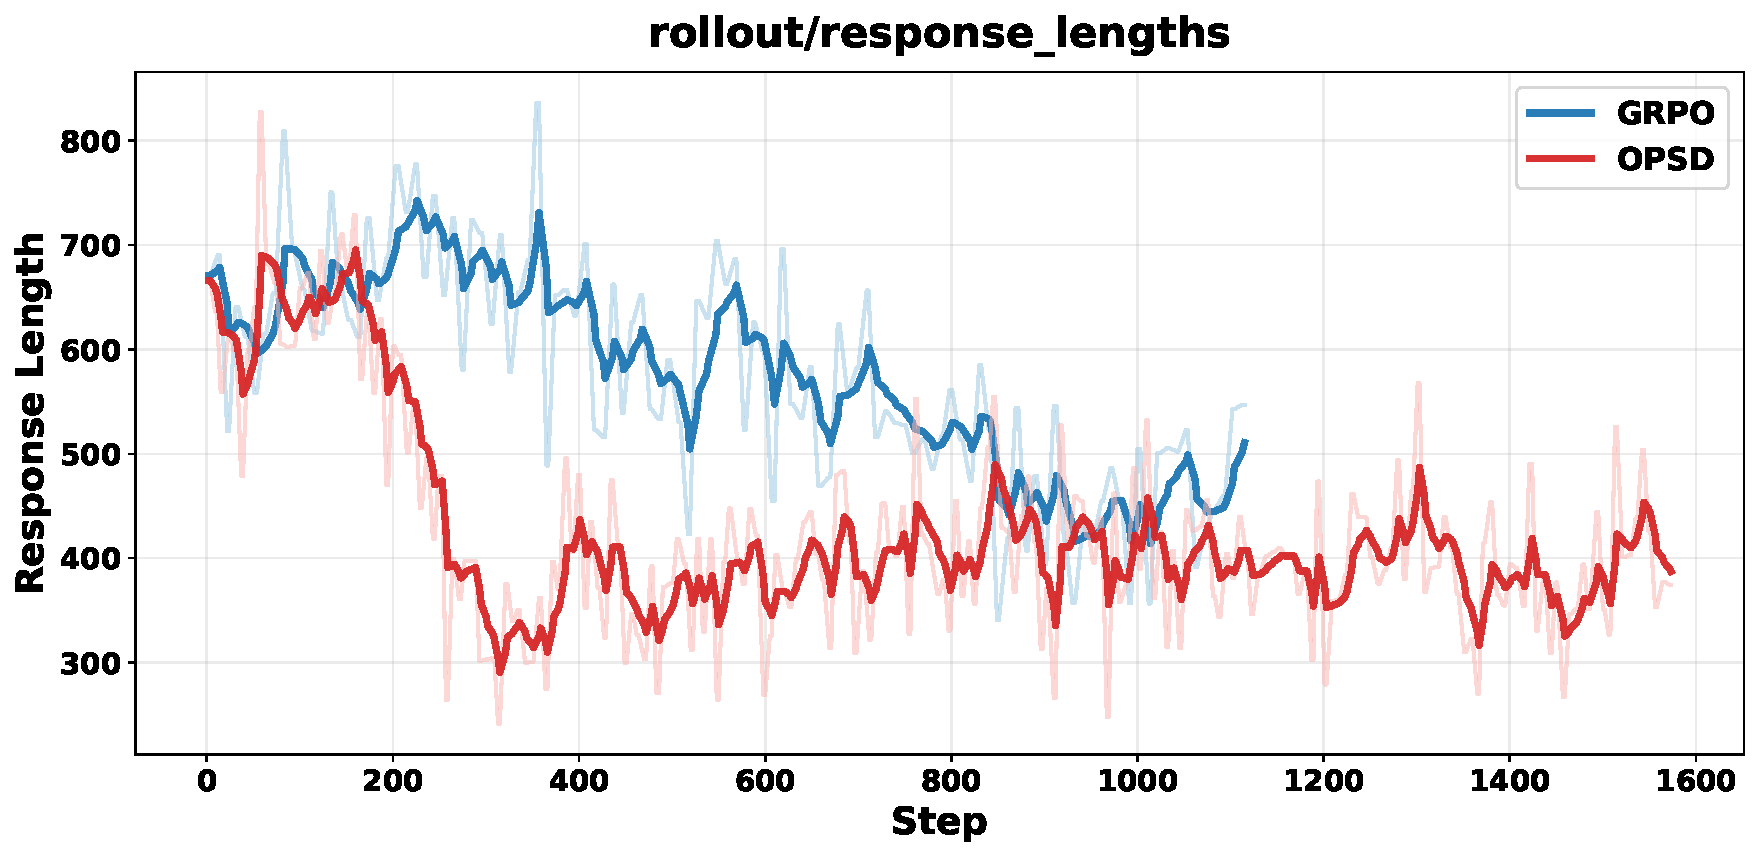
\includegraphics[width=0.3\textwidth]{figures/wildguard_lengths.pdf}
    \hfill
    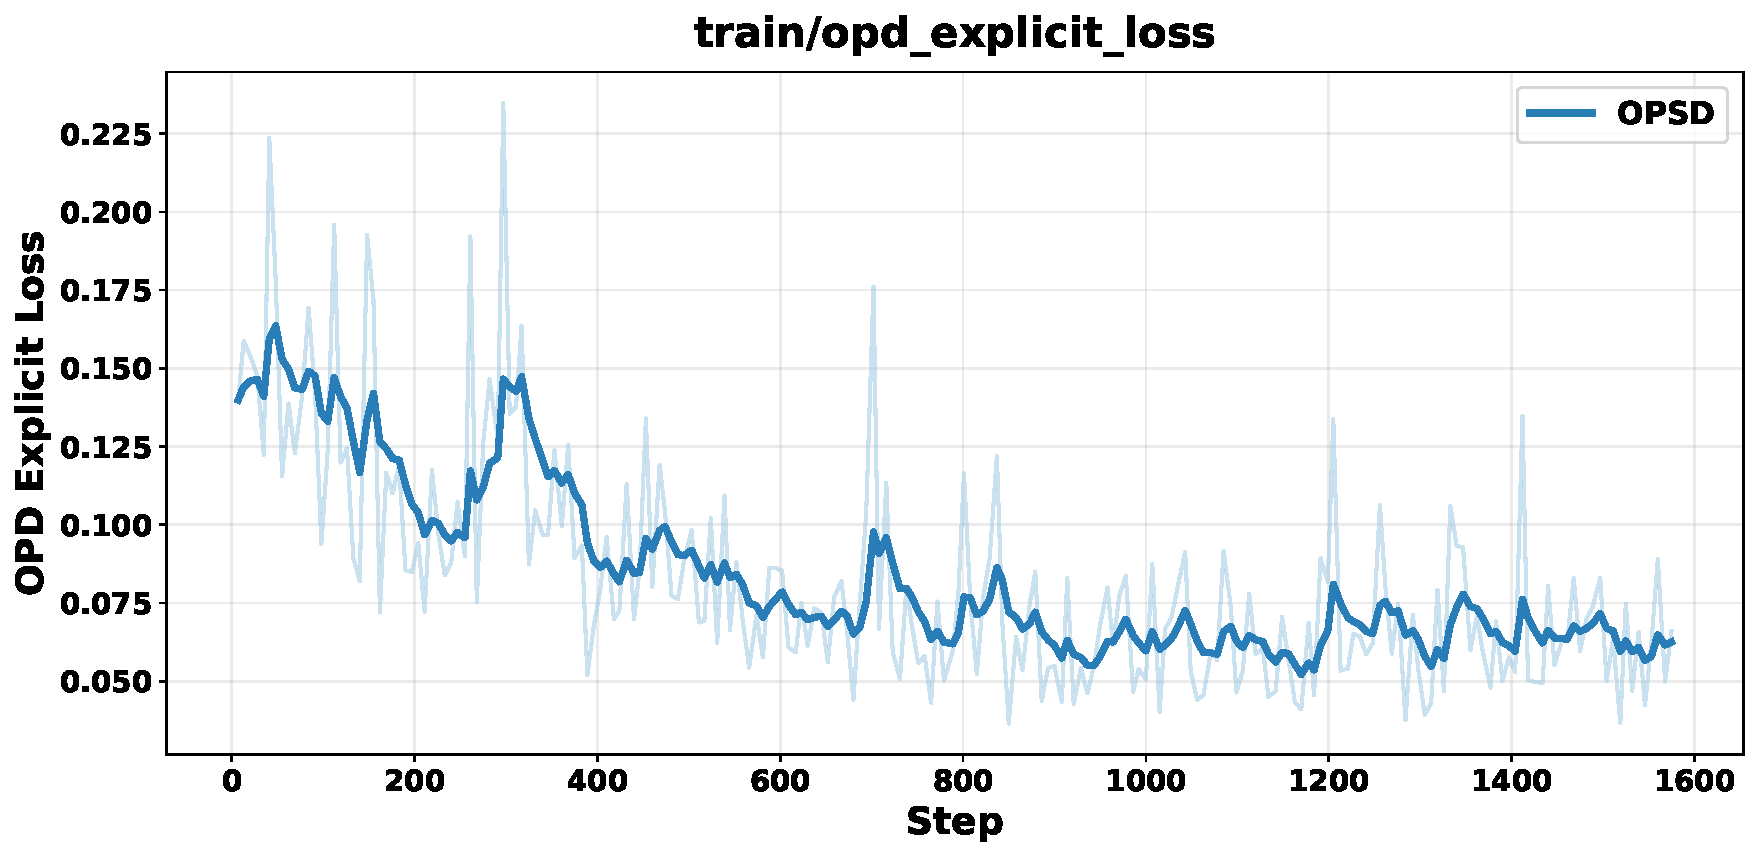
\includegraphics[width=0.3\textwidth]{figures/wildguard_loss.pdf}

    \caption{Train and evaluate Qwen3-1.7B (nothink) on Wildguardmix using their original train and test splits.}
    \label{fig:OPDonwildguard}
\end{figure*}